% ==============================================================================
% SECTION 1: THE LANDSCAPE OF MOBILE-ASSISTED LANGUAGE LEARNING (MALL)
% ==============================================================================
\section{The Landscape of Mobile-Assisted Language Learning (MALL)}
\label{sec:mall_landscape}

    \subsection{Market Evolution and Platform Proliferation}
    \label{subsec:market_evolution}
    Digital language learning platforms (LLPs) have become dominant in foreign language education, with over 70 major commercial applications serving millions of active learners through Mobile-Assisted Language Learning (MALL) \cite{karasimos2022battle}. The scale attained by the market leaders illustrates the extent of this concentration: Duolingo alone reports 58.7 million daily active users and 140.6 million monthly active users as of mid-2026 \cite{duolingo2026q2}. A single platform's design choices therefore shape the learning experience of a substantial share of the world's self-directed language learners, which makes a critical examination of the dominant design paradigm --- rather than only of usage statistics --- a necessary starting point for this thesis.

    This rapid expansion has been further accelerated by Generative Artificial Intelligence (AI) and Large Language Models (LLMs), which have streamlined content authoring and curriculum scaling. While authoring the first 100 language courses on Duolingo required over 12 years of manual pedagogical design, generative models facilitated the deployment of 148 additional courses in early 2025 alone \cite{duolingo2025launch148}. Content authoring is consequently no longer the primary bottleneck to platform growth; as Section~\ref{subsec:platform_limitations} argues, the bottleneck has shifted to \emph{pedagogical design} --- how the abundant, cheaply-generated content is sequenced, contextualised, and reinforced for the individual learner.

    \subsection{Critical Review and Systematic Limitations of Current Platforms}
    \label{subsec:platform_limitations}

    Karasimos \cite{karasimos2022battle} conducted a cross-platform review of five major commercial LLPs --- Duolingo, Memrise, Busuu, LingQ, and Babbel --- evaluated against a fixed set of pedagogical and usability criteria. Although several of these platforms have iterated substantially since that 2022 review, the underlying architectural pattern it identifies --- a static exercise bank gamified with points, streaks, and leaderboards --- remains the dominant paradigm in 2026. Building on that review and on our own examination of the current (2026) state of these five platforms, six systematic limitations recur across the category:

    \begin{enumerate}
        \item \textbf{Uniform Content Delivery Across Learner Demographics and Interests:} Existing platforms deliver static, uniform curricula that do not account for variations in age cohorts (e.g., Gen Z, adults, seniors), communicative objectives, or cultural nuances. Nor do they account for variation in individual \emph{interest}: two learners with identical proficiency levels but distinct interests --- one following football, the other following technology news --- are shown the same fixed exercise bank rather than content drawn from the topics that would sustain their engagement. Machine learning implementations in mainstream platforms focus predominantly on tuning exercise \emph{difficulty} rather than personalising semantic \emph{content} to either dimension \cite{businessresearch2026languageapps}; that is, adaptivity is applied to \emph{how hard} an item is, not to \emph{who it is for} or \emph{what it is about}.

        \item \textbf{Insufficient Multimedia Integration:} Primary instructional routines rely predominantly on isolated text prompts and synthetic text-to-speech audio drills. This structure underutilises the visual and paralinguistic memory channels --- gesture, facial expression, intonation, situational context --- that reinforce natural conversational patterns and prosody, and that a short video clip conveys for free alongside the spoken utterance.

        \item \textbf{Absence of Authentic, Real-World Linguistic Context:} Authentic input --- language produced by native speakers for native speakers within a genuine communicative context, rather than written or graded for pedagogical consumption --- is widely regarded as essential for developing communicative competence, and its use is associated with increased learner motivation and cultural awareness \cite{Gilmore_2007}. Mainstream LLP curricula, by contrast, frequently isolate target vocabulary into synthetic, decontextualised sentences authored specifically for the exercise. Authentic materials are not a costless substitute, however: they routinely presuppose cultural background knowledge that a foreign learner does not yet possess, which can impede comprehension \cite{LiuDong2024AuthenticLanguageModelsClassrooms}. Existing LLPs offer no mechanism through which a confused learner can resolve this kind of gap in situ (Section~\ref{subsec:platform_limitations}, item 6, returns to this point).

        \item \textbf{Shallow Gamification:} Nearly all mainstream platforms are \emph{gamified}, in the sense of layering points, streaks, badges, and leaderboards --- game-design elements --- onto an otherwise conventional drill \cite{deterding2011gamification}. Few, however, qualify as \emph{game-based learning}, in which the learning content is embedded within the core mechanical loop of an actual game rather than merely rewarded by one \cite{plass2015foundations}. Duolingo's exercises, for instance, remain multiple-choice or sentence-construction drills regardless of how many streak-freeze tokens or leaderboard leagues surround them: the reward layer is decorative rather than structural. This distinction matters pedagogically, because points and streaks primarily sustain \emph{extrinsic} engagement (returning to the app), whereas a well-designed game mechanic can additionally scaffold the \emph{cognitive act of retrieval itself}. Section~\ref{subsec:serious_games} develops this distinction as a pedagogical theory; Chapter~\ref{methodology} operationalises it in the design of Glosy's vocabulary-driven games.

        \item \textbf{Limited Advanced Proficiency Support (B2+):} Current mobile platforms focus heavily on A1--B1 grammar foundations, offering sparse resources for upper-intermediate and advanced learners requiring idiomatic fluency, register variation, and natural speech rates. Except for LingQ, which provides authentic content, most platforms fail to support learners meaningfully beyond the B1 level \cite{karasimos2022battle}.

        \item \textbf{Absence of Sociocultural Grounding:} Vygotsky's sociocultural account of cognitive development holds that learning is fundamentally a socially mediated process, not a solitary one (Section~\ref{subsec:sociocultural_theory}) \cite{vygotsky1978mind, lantolf2000sociocultural}. Current mainstream platforms, however, are architected predominantly around single-player, drill-and-feedback loops with limited collaborative scaffolding: a learner who does not understand an idiom or a cultural reference has no in-context avenue to ask a native speaker, a peer, or an instructor. Busuu is a partial exception among the five platforms reviewed here, offering a community feature in which native speakers correct submitted writing and speech samples; this is a genuine sociocultural mechanism, but it is decoupled from the platform's own exercises rather than attached to the specific piece of content the learner is struggling with. Outside the five platforms formally reviewed in this section, dedicated language-exchange applications such as HelloTalk \cite{hellotalk2026} address the social-scaffolding gap directly, connecting learners in real time with native speakers for authentic conversation and correction. This is precisely the gap that authentic materials expose in item 3 above --- authentic content increases the \emph{need} for social scaffolding at exactly the point where a structured, vocabulary-tracking curriculum platform provides the \emph{least} of it --- and it is the gap \textit{Glosy} targets by pairing a tracked vocabulary model with comment-driven, content-attached social scaffolding, identified as future work in Chapter~\ref{chapter:conclusions}.
    \end{enumerate}

    Table~\ref{tab:platform_comparison} summarises the resulting comparative feature matrix, contrasting the five established platforms reviewed above with the design targeted by \textit{Glosy}.

    \begin{table}[htbp]
        \centering
        \small
        \caption{Comparative feature matrix: Established LLPs vs. Glosy framework.}
        \label{tab:platform_comparison}
        \resizebox{\textwidth}{!}{%
        \begin{tabular}{lcccccc}
            \hline
            \textbf{Feature / Dimension}            & \textbf{Duolingo} & \textbf{Memrise} & \textbf{Busuu} & \textbf{Babbel} & \textbf{LingQ} & \textbf{Glosy} \\
            \hline
            Personalized / Interest-Driven Content  & Low               & Low              & Medium         & Medium          & High           & \textbf{High}  \\
            Authentic Multimedia Video              & Low               & Medium           & Medium         & Low             & High           & \textbf{High}  \\
            Deep Gameplay Mechanics                 & Low               & Low              & Low            & Low             & None           & \textbf{High}  \\
            B2+ Proficiency Support                 & Low               & Low              & Medium         & Low             & High           & \textbf{High}  \\
            Adaptive SRS Tracking                   & High              & High             & Medium         & Medium          & Medium         & \textbf{High}  \\
            Sociocultural / Social Scaffolding      & Low               & Low              & Medium         & Low             & Medium         & \textbf{High}  \\
            Open-source                             & No                & No               & No             & No              & No             & \textbf{Yes}   \\
            Novice (A0--A1) Onboarding Ease          & High              & High             & High           & High            & Low            & \textbf{Low}   \\
            \hline
        \end{tabular}%
        }
    \end{table}

    The remainder of this chapter builds the theoretical foundation from which the \textit{Glosy} design responds to each of these six limitations: Section~\ref{sec:pedagogical_foundations} establishes the pedagogical theory, Section~\ref{sec:modalities} reviews the two content modalities (short-form video and serious games) through which that theory is delivered, and Section~\ref{sec:recommendation_algorithms} reviews the algorithmic frameworks that select and sequence content for the individual learner. Section~\ref{sec:synthesis} closes the chapter by mapping each theoretical foundation explicitly onto a corresponding design decision realised in Chapter~\ref{methodology}.


% ==============================================================================
% SECTION 2: PEDAGOGICAL FOUNDATIONS
% ==============================================================================
\section{Pedagogical Foundations}
\label{sec:pedagogical_foundations}

    This thesis follows a \emph{theory-driven design} approach: every major design decision documented in Chapter~\ref{methodology} is traceable to one of the theoretical foundations established in this section, rather than to intuition alone. This section is deliberately scoped to \emph{theory} --- what the literature says about how second language vocabulary is acquired, retained, and forgotten --- and defers the specific computational mechanisms by which \textit{Glosy} operationalises each theory to Chapter~\ref{methodology}, which references back to the relevant subsection below at each design decision.

    \subsection{Sociocultural Theory and the Zone of Proximal Development (ZPD)}
    \label{subsec:sociocultural_theory}
    Vygotsky's Sociocultural Theory posits that cognitive development occurs through socially mediated communication and cultural artefacts, wherein language functions as the primary cognitive tool for organising thought \cite{vygotsky1978mind}. Central to this paradigm is the \textbf{Zone of Proximal Development (ZPD)}: the gap between a learner's independent competence --- what they can accomplish unaided --- and their potential development when assisted by a more capable interlocutor or by structured scaffolding. Lantolf's application of sociocultural theory to second language acquisition (SLA) reframes the ZPD specifically for language learning: instructional stimuli should be pitched neither so far below the learner's current competence that no new learning occurs, nor so far above it that the material is incomprehensible without assistance \cite{lantolf2000sociocultural}. Instructional design is optimal, in this account, precisely at the boundary of what the learner can process with appropriate support.

    The ZPD is a qualitative, dyadic construct: it presupposes a more knowledgeable other (a teacher, a peer, a native speaker) providing scaffolding in real time. Section~\ref{subsec:comprehensible_input} introduces a complementary, quantitative account of the same boundary --- Krashen's Input Hypothesis --- which \textit{Glosy} operationalises computationally in the absence of a live interlocutor (Chapter~\ref{methodology}, Section~\ref{sec:recommendation}). The sociocultural dimension of the ZPD --- social scaffolding through peer or native-speaker interaction --- is not currently implemented in \textit{Glosy}, and is identified as future work in Chapter~\ref{chapter:conclusions} in direct response to the gap identified in Section~\ref{subsec:platform_limitations}, item 6.

    \subsection{The Input Hypothesis and the Lexical Coverage Threshold}
    \label{subsec:comprehensible_input}
    Krashen's Input Hypothesis proposes that language acquisition occurs when a learner is exposed to \emph{comprehensible input} slightly beyond their current competence, denoted $i+1$, where $i$ represents the learner's current linguistic level \cite{krashen1985input}. Input that consists entirely of already-known language ($i$) offers no acquisitional value, while input too far beyond the learner's level ($i+n$, $n \gg 1$) is unparseable and therefore equally unproductive. Although formulated independently of Vygotsky, the Input Hypothesis is widely read alongside sociocultural theory in the SLA literature as a compatible, learner-internal account of the same comprehensibility boundary that the ZPD describes at the level of social interaction \cite{lantolf2000sociocultural}.

    Unlike the ZPD, the $i+1$ boundary admits an empirical, corpus-based operationalisation at the lexical level. Hu and Nation's corpus-based study of unsimplified text established that a reader requires knowledge of approximately 98\% of the running word tokens in a text to comprehend it unaided, with comprehension degrading sharply below that threshold \cite{hunation2000}. This figure was subsequently popularised and synthesised as a general vocabulary-learning target in Nation's widely-cited \textit{Learning Vocabulary in Another Language} \cite{nation2001learning}, and it remains one of the few points at which the largely qualitative construct of comprehensible input admits a precise, machine-checkable definition. This is the specific theoretical result that Chapter~\ref{methodology}, Section~\ref{sec:recommendation} (Stage 1) operationalises as the comprehensibility filter applied to candidate reels.

    \subsection{Cognitive Load Theory and Microlearning}
    \label{subsec:cognitive_load_microlearning}
    Cognitive Load Theory (CLT) holds that working memory capacity is strictly bounded --- classically estimated at $7 \pm 2$ discrete chunks of information \cite{miller1956magical} --- and that instructional design must minimise \emph{extraneous} cognitive load (load imposed by poor presentation, unrelated to the material itself) in order to leave sufficient working-memory capacity for \emph{germane} load, the productive cognitive work of constructing new long-term memory schemata \cite{sweller1988cognitive}. Applied to instructional sequencing, CLT implies that a single learning episode should be bounded in scope: introducing too many new lexical items, grammatical structures, or task demands within one episode exceeds working-memory capacity and displaces schema construction with the effort of merely holding the material in mind.


    \textbf{Microlearning} --- the pedagogical strategy of decomposing instruction into short, self-contained units rather than long-form sessions --- is a direct instructional response to this bound: by construction, a short unit cannot introduce more new material than the working-memory ceiling permits. This principle underlies the length constraints Chapter~\ref{methodology} imposes on both the video content and the game sessions in \textit{Glosy}: each unit of engagement is scoped narrowly enough that the germane load it imposes remains tractable, consistent with the CLT account above.

    \subsection{Memory Decay and Spaced Repetition Models}
    \label{subsec:srs_models}

        \subsubsection{The Ebbinghaus Forgetting Curve}
        \label{subsubsec:ebbinghaus}
        \begin{sloppypar}
        Ebbinghaus's foundational experiments on nonsense-syllable recall demonstrated that memory retention decays over time in the absence of reinforcement, most rapidly immediately after initial exposure and more slowly thereafter \cite{ebbinghaus1885memory}. Although Ebbinghaus's own savings-method data did not yield a single closed-form expression, later reconstructions commonly approximate the resulting \emph{forgetting curve} as a negative exponential function of elapsed time $t$ and a memory-strength parameter $S$: retention $R(t) = e^{-t/S}$, where a larger $S$ corresponds to a more durably consolidated memory. This exponential-decay account is the shared theoretical ancestor of every spaced-repetition model reviewed below: each attempts, with increasing sophistication, to estimate the parameters of an individual learner's own decay curve for an individual item, and to schedule review immediately before predicted recall failure.
        \end{sloppypar}

        \begin{figure}[!htbp]
            \centering
            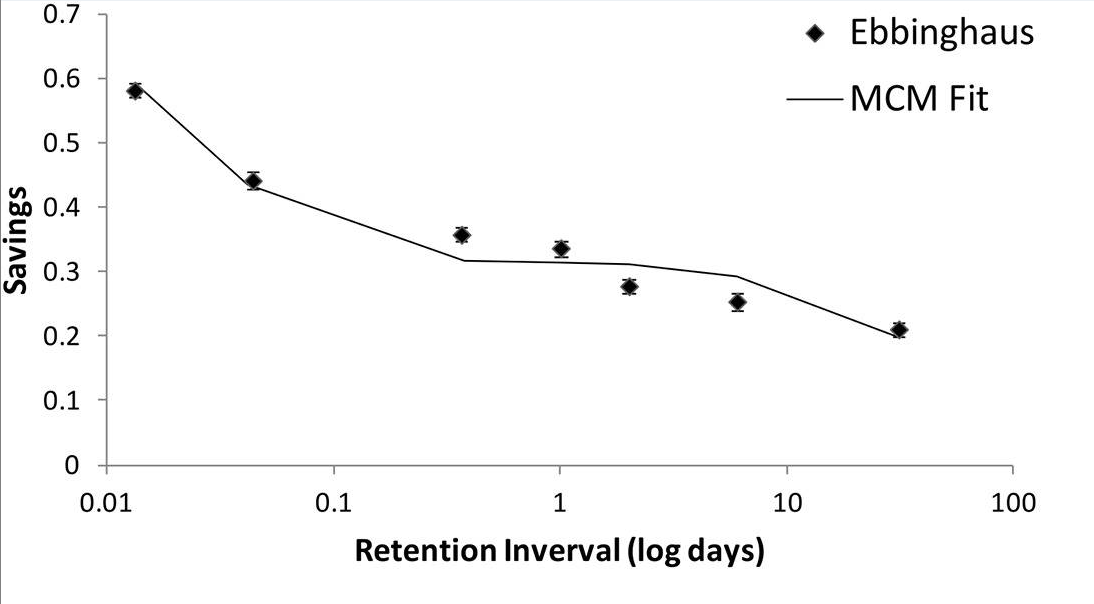
\includegraphics[width=0.60\textwidth]{figures/ebbinghaus_curve.png}
            \caption{The forgetting curve, with original data from Ebbinghaus \cite{ebbinghaus1885memory}, as replotted by Murre and Dros \cite{murre2015replication}. Image: Jaap M. J. Murre, Wikimedia Commons, CC BY 4.0.}
            \label{fig:ebbinghaus_curve}
        \end{figure}

        \subsubsection{Classic Leitner's Algorithm}
        \label{subsubsec:leitner}
        The Leitner system operationalised the forgetting curve as a simple, non-parametric scheduling heuristic decades before it became computationally tractable to fit an individual decay curve per item \cite{leitner1972lernen}. Flashcards are sorted into a series of boxes; a card answered correctly is promoted one box forward, to be reviewed at a longer interval, while a card answered incorrectly is reset all the way back to the first box, regardless of how far it had previously advanced, to be reviewed again at the shortest interval. The scheme requires no numerical memory model at all --- the box number is a coarse, discretised proxy for the item's memory strength $S$ --- which makes it trivially implementable but insensitive to the fact that different items, and different learners, decay at markedly different rates even within the same box.

        \begin{figure}[!htbp]
            \centering
            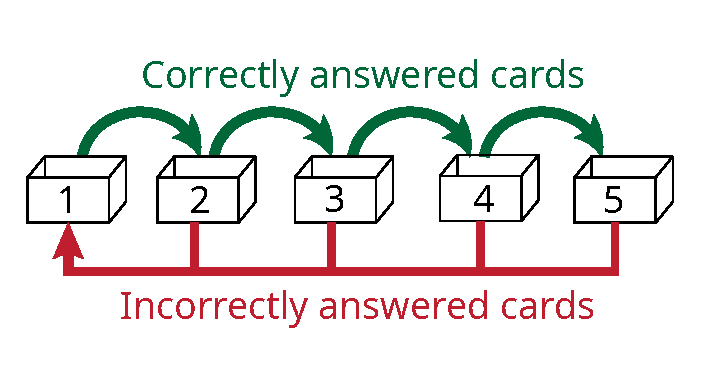
\includegraphics[width=0.62\textwidth]{figures/leitner_system.pdf}
            \caption{The classic five-box Leitner scheduling system. Image: Zirguezi, Wikimedia Commons \cite{zirguezi2012leitner}, CC0 1.0.}
            \label{fig:leitner_system}
        \end{figure}

        \subsubsection{Parametric Half-Life Regression}
        \label{subsubsec:hlr}
        Duolingo's half-life regression (HLR) model, introduced in 2016 \cite{settles2016trainable}, replaces the Leitner system's discrete boxes with a continuous, per-item, per-learner estimate of the memory half-life $h$ --- the elapsed time at which recall probability has decayed to 50\%. Recall probability $p$ for a given item is modelled as an exponential decay in the elapsed interval $\Delta t$ since it was last reviewed, directly generalising the Ebbinghaus curve of Section~\ref{subsubsec:ebbinghaus}:
        \begin{equation}
            \label{eq:hlr_recall}
            p = 2^{-\Delta t / h}
        \end{equation}
        The half-life $h$ itself is not fixed but estimated per item and per learner via a log-linear regression over a feature vector $\mathbf{x}$ --- such as the number of prior correct and incorrect attempts --- with a learned weight vector $\boldsymbol{\Theta}$:
        \begin{equation}
            \label{eq:hlr_halflife}
            \hat{h}_{\boldsymbol{\Theta}}(\mathbf{x}) = 2^{\boldsymbol{\Theta} \cdot \mathbf{x}}
        \end{equation}
        generalising the Leitner box index into a continuously-valued, learner- and item-specific quantity. The weight vector $\boldsymbol{\Theta}$ is not known in advance: it must itself be fitted offline, by regression over a large historical corpus of review outcomes pooled across many users, before Equation~\ref{eq:hlr_halflife} can be applied to a single new one --- Settles and Meeder trained their original model on Duolingo's own multi-million-user interaction log \cite{settles2016trainable}. A newly-launched application, without an equivalent corpus of prior review data from which to fit $\boldsymbol{\Theta}$, cannot reproduce this regression from its own history alone. Section~\ref{subsubsec:fsrs} reviews an alternative memory model that avoids this cold-start requirement.

        \subsubsection{FSRS and the DHP Model}
        \label{subsubsec:fsrs}
        The Free Spaced Repetition Scheduler (FSRS) originates in the DHP model developed at MaiMemo \cite{ye2022stochastic}, a variant of what the open-source scheduling community terms the \textbf{DSR} model: memory state is represented not by a single half-life $h$, as in HLR, but by three jointly-updated variables --- \textbf{difficulty} $D \in [1, 10]$ (how intrinsically hard the item is to learn), \textbf{stability} $S$ (the number of days for retrievability to decay to 90\%), and \textbf{retrievability} $R$ (the instantaneous, momentary probability of successful recall, analogous to $p$ in HLR). Each is revised after every individual review rather than re-estimated from scratch, and each review is scored on a four-point grade $G \in \{1,2,3,4\}$ (\emph{again}, \emph{hard}, \emph{good}, \emph{easy}). Since its first release, FSRS has been refined through several major versions (v1 through the current FSRS-6), each adding parameters and improving the empirical fit of its forgetting curve and update rules \cite{opensr2026algorithm}; the formulation below is the current one (FSRS-6), noting where it revises earlier versions.

        \paragraph{The forgetting curve.} Rather than the fixed exponential decay of Equation~\ref{eq:hlr_recall}, FSRS models retrievability as a power-law function of the elapsed interval $t$ and the current stability $S$, with a trainable decay exponent $w_{20}$ (the $w_i$ denote the elements, $0$-indexed, of a fitted 21-parameter weight vector $\mathbf{w}$):
        \begin{equation}
            \label{eq:fsrs_retrievability}
            R(t, S) = \left(1 + \text{factor} \cdot \frac{t}{S}\right)^{-w_{20}}, \qquad \text{factor} = 0.9^{-1/w_{20}} - 1,
        \end{equation}
        where the factor term is chosen precisely so that $R(S, S) = 0.9$ always holds, preserving stability's definition regardless of the fitted value of $w_{20}$. This is itself the product of two earlier simplifications: the original FSRS v4 fixed the exponent at $w_{20}=1$ with $\text{factor}=1/9$, reducing Equation~\ref{eq:fsrs_retrievability} to $R(t,S) = (1 + t/9S)^{-1}$; FSRS-4.5 refined this to a fixed exponent of $0.5$; only from FSRS-5 onward is the decay shape itself learned from data.

        \paragraph{Initial state and difficulty updates.} A word's very first review initialises stability and difficulty directly from the grade it receives:
        \begin{equation}
            \label{eq:fsrs_initial}
            S_0(G) = w_{G-1}, \qquad D_0(G) = w_4 - e^{w_5 (G-1)} + 1,
        \end{equation}
        so that, for instance, an item first rated \emph{again} ($G=1$) starts at the lowest stability $w_0$ and the highest difficulty $D_0(1) = w_4$. On every subsequent review, difficulty drifts by a grade-dependent increment and is then pulled back towards a fixed target via \emph{mean reversion}:
        \begin{equation}
            \label{eq:fsrs_difficulty}
            D' = D - w_6 (G - 3) \cdot \frac{10 - D}{9}, \qquad D'' = w_7 \, D_0(4) + (1 - w_7) \, D',
        \end{equation}
        anchoring difficulty to $D_0(4)$ (the initial difficulty of an \emph{easy}-rated item) rather than letting it drift unboundedly after a long run of easy or hard grades --- informally termed avoiding ``ease hell'' in the flashcard-scheduling community.

        \paragraph{Stability updates.} Following a successful review ($G \in \{2,3,4\}$), stability increases according to
        \begin{equation}
            \label{eq:fsrs_stability_recall}
            S_r'(D, S, R, G) = S \cdot \Big(e^{\,w_8 (11 - D) \, S^{-w_9} \left(e^{w_{10}(1-R)} - 1\right) \cdot w_{15}^{[G=2]} \cdot w_{16}^{[G=4]}} + 1\Big),
        \end{equation}
        while a lapse ($G=1$) instead resets stability to a smaller post-lapse value,
        \begin{equation}
            \label{eq:fsrs_stability_forget}
            S_f'(D, S, R) = w_{11} \, D^{-w_{12}} \left((S+1)^{w_{13}} - 1\right) e^{w_{14}(1-R)}.
        \end{equation}
        Writing $S_{\mathrm{inc}} = S_r'/S$ for the multiplicative stability gain of a successful review, three qualitative properties of Equation~\ref{eq:fsrs_stability_recall} recur throughout the FSRS documentation and are directly interpretable in terms of the theory already established in this chapter: $S_{\mathrm{inc}}$ decreases as difficulty $D$ increases (harder items consolidate more slowly); $S_{\mathrm{inc}}$ decreases as stability $S$ itself increases (an already well-consolidated memory is harder to strengthen further, consistent with the diminishing-returns shape of the Ebbinghaus curve in Section~\ref{subsubsec:ebbinghaus}); and $S_{\mathrm{inc}}$ increases as retrievability $R$ decreases at the time of review, i.e.\ a successful recall of an \emph{almost-forgotten} item strengthens memory more than reviewing an item that was never at risk --- the computational signature of the spacing effect.

        \paragraph{Same-day reviews (FSRS-6).} The formulas above govern reviews spaced at least a day apart. FSRS-6's specific contribution is a separate, more conservative update for a card reviewed again on the same day it was last seen:
        \begin{equation}
            \label{eq:fsrs_stability_sameday}
            S'(S, G) = S \cdot e^{\,w_{17}(G - 3 + w_{18}) \, S^{-w_{19}}},
        \end{equation}
        which grows quickly while $S$ is still small and flattens as $S$ grows, converging once $S_{\mathrm{inc}} = e^{w_{17}(G-3+w_{18})S^{-w_{19}}} = 1$; earlier versions used the same functional form without the $S^{-w_{19}}$ damping term, allowing same-day repetition to inflate stability unrealistically.

        This finer-grained decomposition is, at the time of writing, the most empirically accurate publicly documented model of spaced-repetition scheduling. Critically for a new application, all of Equations~\ref{eq:fsrs_retrievability}--\ref{eq:fsrs_stability_sameday} update the per-item state \emph{incrementally, after each individual review}, using a fixed parametric rule rather than a regression re-fitted in a single offline pass over a large historical corpus, as HLR requires (Section~\ref{subsubsec:hlr}). A new item begins from the initial-state Equation~\ref{eq:fsrs_initial} and refines its own difficulty and stability purely from the learner's own subsequent review history, without needing Duolingo-scale historical data first; \textit{Glosy} adopts the published default parameter vector $\mathbf{w}$ rather than fitting its own, precisely because it does not yet have the review corpus such a fit would require. This is the specific reason Chapter~\ref{methodology}, Section~\ref{sec:recommendation} (Stage 2) adopts the FSRS formulation, rather than HLR, as the basis of the \texttt{SRS\_Urgency} scoring term in the recommendation engine: a word's recommendation urgency rises as its predicted retrievability $R$ (Equation~\ref{eq:fsrs_retrievability}) falls.

    \subsection{Active Recall and the Testing Effect}
    \label{subsec:testing_effect}
    A separate, complementary strand of cognitive psychology addresses not \emph{when} to review an item, but \emph{how}. The testing effect --- robustly demonstrated across decades of memory research --- shows that the act of actively retrieving an item from memory (as in a test or a recall task) produces substantially better long-term retention than an equivalent amount of time spent passively re-studying the same item \cite{roediger2006testing}. This finding motivates a specific design constraint distinct from, and additional to, the scheduling question addressed by Section~\ref{subsec:srs_models}: \emph{when} an item is due for review, the review task itself should require productive retrieval (e.g., recalling and typing a word) rather than passive recognition (e.g., selecting a familiar-looking option among distractors). Section~\ref{subsec:serious_games} reviews game mechanics through this lens.


% ==============================================================================
% SECTION 3: MODALITIES FOR ACQUISITION AND ACTIVE REINFORCEMENT
% ==============================================================================
\section{Modalities for Language Acquisition}
\label{sec:modalities}

    Sections~\ref{subsec:comprehensible_input}--\ref{subsec:testing_effect} establish \emph{what} an effective input and reinforcement episode should look like theoretically: comprehensible ($i+1$), authentic, cognitively bounded, spaced, and actively recalled. This section reviews the empirical literature on the two content modalities through which \textit{Glosy} delivers input and reinforcement respectively: short-form video, addressed to the input side of acquisition, and serious games, addressed to the active-recall side.

    \subsection{Short-Form Video in Second Language Acquisition (SLA)}
    \label{section:reels_in_sla}

        \subsubsection{Incidental Vocabulary Acquisition through Audiovisual Input}
        A substantial body of research in Computer-Assisted Language Learning (CALL) predates the short-form video format itself and concerns the closely related case of captioned television and film viewing. Vanderplank's early work on teletext subtitles found that captioned video supports vocabulary and listening development beyond what audio alone provides, by allowing the learner to cross-reference the written and spoken forms of an unfamiliar item in real time \cite{vanderplank1988value}. More recent corpus-informed work confirms this incidental-learning effect at scale: Peters and Webb found measurable incidental vocabulary gains from watching L2 television programmes without any explicit study task, with gains moderated by frequency of item occurrence and by the presence of captions \cite{peters2018incidental}, while Montero Perez, Peters, and Desmet found that enhancing target vocabulary within video captions (e.g., through highlighting) further improves retention relative to unenhanced captioned video \cite{monteroperez2018vocabulary}. Taken together, this literature establishes that passive audiovisual viewing is a genuine, if modest, channel of incidental vocabulary acquisition, and that the effect is strengthened, not weakened, by textual scaffolding synchronised to the audio track --- precisely the token-level, timestamped transcript structure that a \textit{Glosy} reel provides (Chapter~\ref{methodology}, Section~\ref{sec:data_modelling}).

        \subsubsection{The Gap: Passive Consumption without Reinforcement}
        \label{subsubsec:passive_consumption_gap}
        The incidental-acquisition literature reviewed above is consistent in one further respect: the vocabulary gains it reports from passive viewing alone are real but small, typically requiring many repeated incidental encounters of an item before it is durably retained \cite{peters2018incidental}. Passive viewing, in other words, is an effective delivery mechanism for comprehensible input (Section~\ref{subsec:comprehensible_input}) but is not, by itself, a spaced-repetition system in the sense of Section~\ref{subsec:srs_models}: a viewer has no mechanism by which an encountered item is tracked, scheduled for review, or actively retrieved once the video ends. This is the specific gap in generic short-form social video consumption --- as opposed to a purpose-built application --- that motivates the research question posed in Chapter~\ref{chapter:intro}: watching unstructured reels on an existing social platform provides input without a tracked vocabulary state, and therefore without the scheduled, active-recall reinforcement that Sections~\ref{subsec:srs_models} and~\ref{subsec:testing_effect} identify as necessary for durable retention. Closing this gap requires attaching a conventional SRS review step --- of the kind ordinarily triggered by a static flashcard in an application such as Anki --- directly to the moment a due item is encountered inside a reel, rather than leaving that encounter to pass by unrecorded. Chapter~\ref{methodology} details the interface through which \textit{Glosy} does this: a due word appearing in a reel's transcript prompts an in-context review step immediately after viewing, through which the learner's recall grade $G$ is captured and fed into the FSRS update rules of Section~\ref{subsubsec:fsrs} (Equations~\ref{eq:fsrs_stability_recall}--\ref{eq:fsrs_stability_forget}) --- the reel itself standing in for the static flashcard as the review's triggering stimulus.

    \subsection{Serious Games and Gamification in Language Learning}
    \label{subsec:serious_games}

        \subsubsection{Game-Based Learning versus Gamification}
        \label{subsubsec:gbl_vs_gamification}
        Section~\ref{subsec:platform_limitations} (item 4) distinguished \emph{gamification} --- decorating an existing task with game-design elements such as points and streaks \cite{deterding2011gamification} --- from \emph{game-based learning}, in which the instructional content is embedded within the mechanical loop of an actual game \cite{plass2015foundations}. This distinction is well established as a specific research strand within CALL: Godwin-Jones's review of games in language learning documents a persistent gap between the two, noting that commercially successful language-learning products have historically favoured drill-based gamification because it is comparatively cheap to build and easy to monetise, while games in which linguistic competence is itself the win condition remain comparatively rare \cite{godwinjones2014games}. Sykes and Reinhardt's broader treatment of digital games in second and foreign language teaching similarly argues that a game's pedagogical value derives from whether target-language production or comprehension is load-bearing to \emph{winning the game}, not merely rewarded upon completion of an unrelated exercise \cite{sykes2013language}.

        \subsubsection{Difficulty Adaptation in Hypercasual Games}
        \label{subsubsec:dda}
        Section~\ref{sub:hypercasual_and_hybrid_casual_games} (Chapter~\ref{chapter:intro}) established the hypercasual genre's core appeal: minimal onboarding, immediately intuitive mechanics, and short session length --- properties that align closely with the microlearning argument of Section~\ref{subsec:cognitive_load_microlearning}. Within game design more specifically, dynamic difficulty adjustment (DDA) --- algorithmically tuning a hypercasual game's difficulty in response to the individual player's observed performance, rather than fixing it in advance --- has been shown to improve player retention and perceived replay value relative to a static difficulty curve \cite{yang2020hyper}. This provides the game-design-theoretic counterpart to the lexical personalisation argument of Section~\ref{sec:recommendation_algorithms}: just as a reel should be selected for lexical comprehensibility, a game level's difficulty should be tuned to the player's demonstrated skill --- in \textit{Glosy}'s case, the specific vocabulary items the level is built from, rather than a generic difficulty parameter.

        \subsubsection{Active-Recall Game Mechanics for Vocabulary}
        \label{subsubsec:active_recall_games}
        The testing-effect literature reviewed in Section~\ref{subsec:testing_effect} \cite{roediger2006testing} favours game mechanics that require \emph{productive} retrieval of a target word's orthographic form over mechanics that require only its \emph{recognition} among distractors. Word-reconstruction puzzle formats --- in which the player must recall and produce a target word letter-by-letter, validating each attempt against positional or compositional constraints --- structurally enforce this kind of active retrieval as the core win condition of the game itself, rather than as an optional or bypassable step. This is the specific theoretical property, rather than genre popularity alone, that motivates the word-reconstruction game modalities implemented in \textit{Glosy} and documented in Chapter~\ref{methodology}, Section~\ref{sec:games_design}.


% ==============================================================================
% SECTION 4: ALGORITHMIC FRAMEWORKS FOR PERSONALIZED RECOMMENDATION
% ==============================================================================
\section{Algorithmic Frameworks for Personalized Recommendation}
\label{sec:recommendation_algorithms}

    Sections~\ref{sec:pedagogical_foundations} and~\ref{sec:modalities} establish \emph{which} content is pedagogically appropriate for a learner at a given moment: comprehensible (Section~\ref{subsec:comprehensible_input}), due for review (Section~\ref{subsec:srs_models}), and appropriately reinforcing (Section~\ref{sec:modalities}). Selecting such content automatically, per learner, is a recommendation problem in the information-retrieval sense. This section reviews the two classical recommendation paradigms, content-based and collaborative filtering, and the strategies the literature offers for combining them; Section~\ref{sec:synthesis} maps this theory onto \textit{Glosy}'s own recommendation engine.

    \subsection{Content-Based Filtering}
    \label{subsec:content_based_filtering}
    Content-based filtering recommends items by comparing an item's own features against a profile of a single user's own preferences, built from that user's history, without reference to other users' behaviour \cite{adomavicius2005toward}. Its principal known limitation is that it has no way to express a temporal signal such as \emph{when} a previously-seen item is due for review \cite{adomavicius2005toward} --- a gap the memory-decay models of Section~\ref{subsec:srs_models} are specifically designed to fill.

    \subsection{Collaborative Filtering and Hybrid Recommender Systems}
    \label{subsec:cascade_hybrid}
    Collaborative filtering (CF) recommends items based on patterns of agreement across many users' behaviour --- favouring items that users with a similar engagement history have responded well to --- rather than on an item's own features \cite{adomavicius2005toward}. Because it depends on an interaction matrix populated across many users, CF is known to perform poorly under the \emph{cold-start} problem, when a system has few users or little accumulated interaction history \cite{adomavicius2005toward}.

    Burke's survey of hybridisation strategies for combining multiple recommendation techniques distinguishes several ways of doing so, including \emph{weighted} hybridisation, in which each technique produces an independent score and the final score is their linear combination, and \emph{cascade} hybridisation, in which one technique coarsely ranks or partitions the candidate set and a second technique is applied only to break ties within it \cite{burke2002hybrid}. Ricci et al.'s handbook situates both strategies, and content-based and collaborative filtering more generally, within the broader design space of recommender systems \cite{ricci2011introduction}.

    \subsection{Recommender Systems in Educational Technology}
    \label{subsec:edtech_recommenders}
    Recommender systems applied to e-learning typically personalise the sequencing of resources or exercise \emph{difficulty} to a learner's inferred ability, rather than the semantic content of what is recommended \cite{klasnja2011elearning} --- the same gap identified in Section~\ref{subsec:platform_limitations} (item~1).


% ==============================================================================
% SECTION 5: SYNTHESIS -- A THEORY-DRIVEN DESIGN FRAMEWORK
% ==============================================================================
\section{Synthesis: A Theory-Driven Design Framework}
\label{sec:synthesis}

    This chapter has reviewed, in turn, the pedagogical theory of comprehension and retention (Section~\ref{sec:pedagogical_foundations}), the empirical literature on the two content modalities through which \textit{Glosy} delivers input and reinforcement (Section~\ref{sec:modalities}), and the algorithmic frameworks by which content is selected and sequenced for the individual learner (Section~\ref{sec:recommendation_algorithms}). Table~\ref{tab:theory_synthesis} makes explicit the traceability between each theoretical foundation reviewed above and the corresponding design decision it motivates in Chapter~\ref{methodology}, operationalising the theory-driven design approach stated at the outset of Section~\ref{sec:pedagogical_foundations}.

    \begin{table}[htbp]
        \centering
        \small
        \caption{Theory-driven design traceability matrix: theoretical foundation, design implication, and the corresponding Glosy component.}
        \label{tab:theory_synthesis}
        \begin{tabular}{p{3.6cm}p{4.6cm}p{4.6cm}}
            \hline
            \textbf{Theoretical Foundation} & \textbf{Design Implication} & \textbf{Glosy Component} \\
            \hline
            ZPD (\ref{subsec:sociocultural_theory}) \& Input Hypothesis (\ref{subsec:comprehensible_input}) &
            Recommend content at the $i+1$ comprehensibility boundary &
            Stage 1: Comprehensibility Filtering, 98\% lexical coverage (Sec.~\ref{subsec:stage1_design}) \\
            \hline
            Cognitive Load Theory \& Microlearning (\ref{subsec:cognitive_load_microlearning}) &
            Bound each learning episode to a short, self-contained unit &
            90-second reel cap; Wordle attempt limit; Word of Wonders word/letter caps (Sec.~\ref{sec:system_overview}, Sec.~\ref{sec:games_design}) \\
            \hline
            Forgetting Curve \& Spaced Repetition (\ref{subsec:srs_models}) &
            Schedule review before predicted recall failure &
            Stage 2: Spaced-Repetition Prioritisation, due-word partitioning (Sec.~\ref{subsec:stage2_design}) \\
            \hline
            Testing Effect (\ref{subsec:testing_effect}) \&
            Game-Based Learning (\ref{subsec:serious_games}) &
            Require productive retrieval, not passive recognition &
            Wordle-style and Word of Wonders vocabulary games (Sec.~\ref{sec:games_design}) \\
            \hline
            Cascade Hybrid Recommender (\ref{subsec:cascade_hybrid}) &
            Filter by comprehensibility, partition by due-for-review, break ties by engagement-weighted content similarity &
            Stage 1--3 cascade ranking (Sec.~\ref{subsec:cascade_design}) \\
            \hline
            Sociocultural Theory (\ref{subsec:sociocultural_theory}) &
            Provide social scaffolding for culturally-opaque authentic input &
            Collaborative learning features (Ch.~\ref{chapter:conclusions}, Future Work) \\
            \hline
        \end{tabular}
    \end{table}

    Read together with the platform limitations identified in Section~\ref{subsec:platform_limitations}, this synthesis reframes the research questions posed in Chapter~\ref{chapter:intro} as a design problem with a specific theoretical answer for each of its parts: RQ1 is addressed by the content-based lexical filtering of Section~\ref{subsec:content_based_filtering} operating over the short-form video modality of Section~\ref{section:reels_in_sla}; RQ2 is addressed by the cascade hybrid of Section~\ref{subsec:cascade_hybrid}, fusing comprehensibility with the memory-decay models of Section~\ref{subsec:srs_models}; and RQ3 is addressed by the active-recall game theory of Section~\ref{subsec:serious_games}, parameterised by the same memory-decay state that governs RQ2. Chapter~\ref{methodology} now presents the system architecture that implements this framework.

\newpage
